% Discription of what is a Artificial Neural Networks and what does it
\chapter{Artificial Neural Networks\authorB}

\section{What is a Artificial Neural Networks?}

  \textbf{A}rtificial \textbf{N}eural \textbf{N}etworks(ANN) are inspired by biological neural networks that constitute animal brains. Important to notice is that they are not faithful models of biologic neural or cognitive phenomena. In fact most of these models are more closely related to mathematical and/or statistical models(For Example: clustering algorithms). Such systems "learn" to perform tasks by considering examples, generally without being programmed with task-specific rules. 
 
\section{Areas of Application}

 ANN are viable computational models for a wide variety of problems, including pattern classification, speech synthesis and recognition, adaptive interfaces between human and complex physical system, function approximation, associative memory, clustering, forecasting and prediction, combinatorial optimization, nonlinear system modeling, and control
 \cite{fundamentals_ann}
 
\section{Components of an ANN}

Simplified a ANN consists of these components: neurons, connection and the weight associated with them, the propagation function, a loss function and a bias. The following topics will give you a short summary what these components are and afterward is an explanation  how they work together. 

\subsection{Neurons}

Neurons are elementary units in an ANN. A neuron gets one ore more inputs and depending on the value of the inputs the output is set. A neuron can get its inputs from other neurons or, if its at the beginning, from the source of the data that needs to be processed. Depending on the Type of ANN they are placed in different structures. In most cases the output of a Neuron is a number between 0 and 1.

\begin{figure}[h]
	\centering
	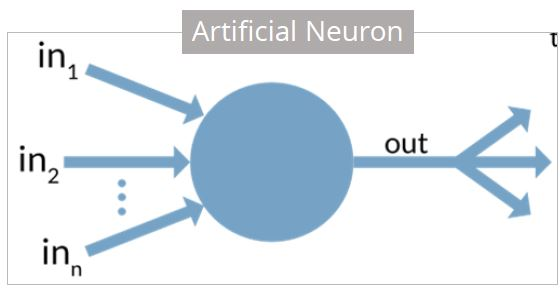
\includegraphics[width=0.7\textwidth]{./media/images/diagram-for-general-view-of-artificial-neuron.jpg}
  	\caption{General view of Neurons
  	\\Source: https://tinyurl.com/yyfthk7c}
  	\label{Gvon}
\end{figure}

\subsection{Connection and weights}

These Neurons are Connected. Which neurons are connected with others depends on the structure. The weights characterize how important a connection between neurons is. 

\textbf{For example:}\newline
A neuron, we call it base for this example, has two neurons connected to it as inputs. The weight of the connection of the first neuron has a bigger weight than the second connection. That means the output of the base depends more on the input of the first neuron 

\subsection{Propagation function  and activation function}

This is a function witch takes the Inputs of a neuron, the weight of these connections and the bias and adds them up. The resulting value is the processed by the activation function which sets the output. One of the most common activation function is the sigmoid function because it is not a step function which means the output does not  change instantaneously. That is important for the training algorithm.

\subsection{Bias}

The bias is a Neuron which has no Inputs. A bias is used to shift the decision boundary to the left or right.

\section{Organization}

A artificial neural network can be organized in many different ways.

\subsection{Feed Forward ANN}

\begin{figure}[h]
	\centering
	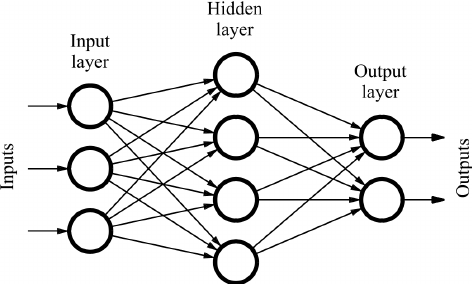
\includegraphics[width=0.7\textwidth]{./media/images/feed_forward_neural_network.png}
  	\caption{Feed forward network}
  	\label{ffNN}
\end{figure}

The following picture demonstrates a feed forward ANN .There are a variable number of hidden layers depending on the purpose of the neural network. Nothing in the hidden layer is visible. 

\subsection{CNN}

Convolution Neural Network (CNN) is the most important Network organization for this task. It is based on the human visual cortex and perfect for image and video recognition. The components of a CNN are a series of convolution and sub-sampling layers followed by a fully connected layer and a normalizing layer.

How a CNN works will be explained in the following example. The same example like in "Review of Deep Learning Algorithms and Architectures"\cite{networks,exampleCNN} will be used
\begin{figure}[h]
	\centering
	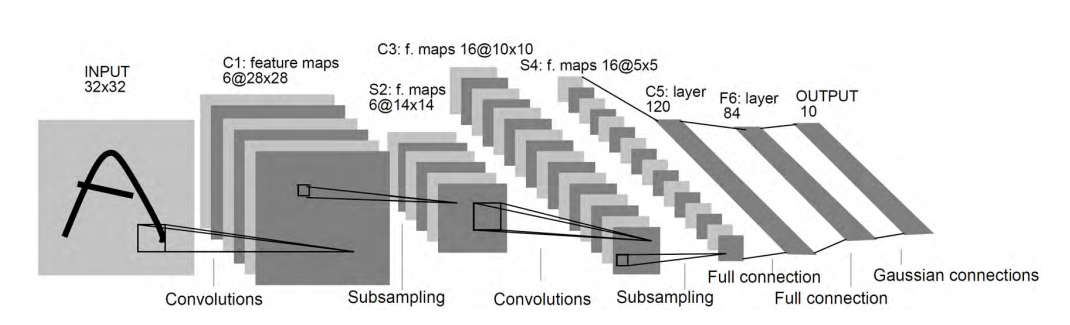
\includegraphics[width=1.1\textwidth]{./media/images/CNN.PNG}
  	\caption{7-layer architecture of CNN for character recognition
  	\\ \cite[Fig.~4.]{networks,exampleCNN}}
  	\label{CNN}
\end{figure}

Progressively more refined feature extraction at every layer is performed by the series of multiple convolution layers. This process is moving from input to output layer. After the convolution layers there are fully connected layers that perform classification. There is also the possibility of putting Sub-sampling or pooling layers between each convolution layer. The input of a CNN is a 2D n*n pixelated image. Each layer consists of filters or kernels (groups of 2D neurons). In most neural networks neurons in each feature extraction layer are connected to all neurons in the adjacent layers. But in a CNN they are only connected to the spatially mapped fixed sized and partially overlapping neurons in the previous layer’s input image or feature map.

\section{Encoder-Decoder-Based Architecture}

Encoder-Decoder-Based networks are networks, which try to reconstruct their own input. You construct the network so that it reduces the input size by using one or more hidden layers, until it reaches a reasonably small hidden layer in the middle. As a result your data has been compressed (encoded) into a few variables. From this hidden representation the network tries to reconstruct (decode) the input again.

In order to do a good job at reconstructing the input the network has to learn a good representation of the data in the middle hidden layer. This can be useful for dimensionality reduction, or for generating new “synthetic” data from a given hidden representation. This is especially important considering that we are trying to construct a 3D Map out of the Camera Input. 









